\documentclass[a4paper,12pt]{article}
\usepackage[utf8]{inputenc}
\usepackage{amsmath}
\usepackage{amsfonts}
\usepackage{amssymb}
\usepackage{graphicx}
\usepackage{hyperref}
\usepackage{geometry}
\usepackage{fancyhdr}
\usepackage{subcaption}

\newcommand{\auth}{Pranav Chandra N. V.}
\newcommand{\titleinfo}{EEE F313: ADVD Lab 3 Report}
\newcommand{\id}{2023AAPS0013}

\pagestyle{fancy}
\fancyhf{}
\renewcommand{\headrulewidth}{0.4pt} % full-width rule
\fancyhead[L]{\titleinfo}
\fancyhead[R]{\auth}
\fancyfoot[C]{\thepage}

\geometry{a4paper, margin=1in}
\title{\titleinfo}
\author{\auth \\ \id}
\date{}

\begin{document}
\maketitle
\section{Introduction}
This lab had the goal of performing both static and transient analysis on a CMOS inverter. The CMOS inverter circuit is shown below in Figure \ref{fig:cmos-circuit}.
\begin{figure}[h!]
	\centering
	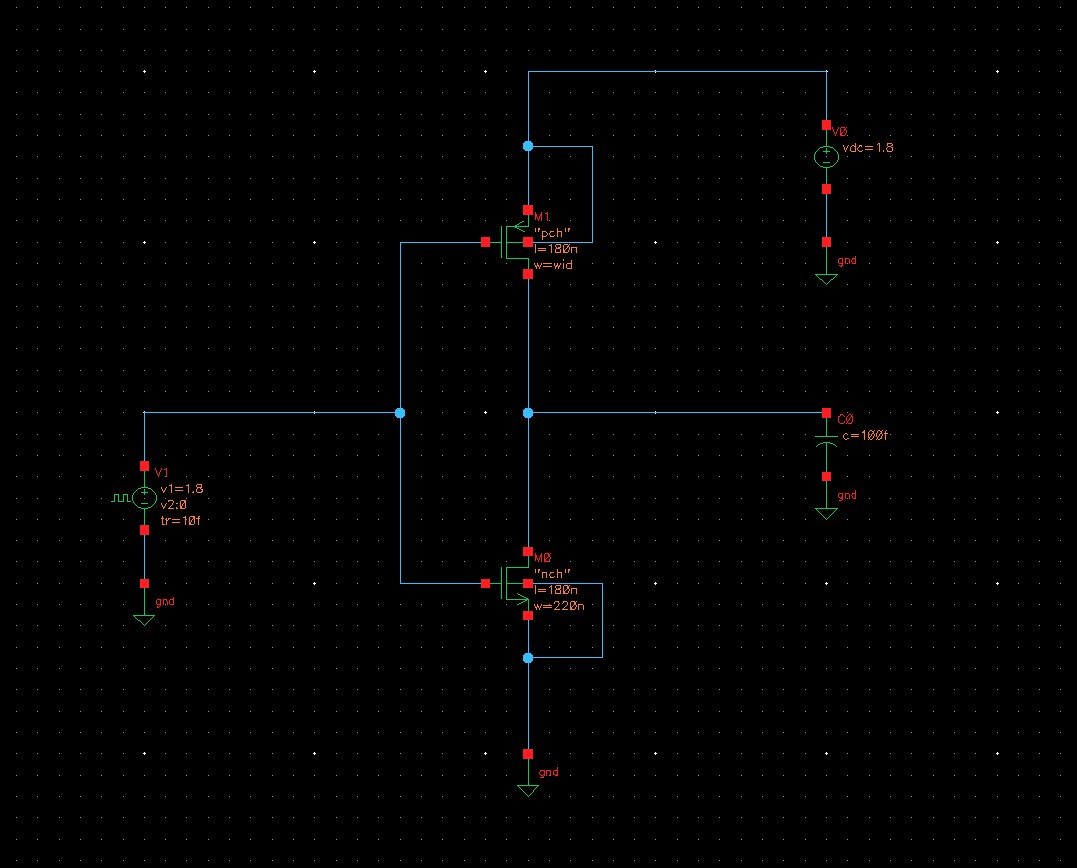
\includegraphics[width=0.8\textwidth]{images/cmos-circuit.png}
	\caption{CMOS Inverter Circuit}
	\label{fig:cmos-circuit}
\end{figure}

\newpage
\section{Identifying CMOS Inverter Parameters}
From the CMOS circuit in Figure \ref{fig:cmos-circuit}, the following parameters were identified by plotting the VTC curve and it's derivative in Cadence. Both the curves are shown below in Figures \ref{fig:vtc_curve} and \ref{fig:vtc_derivative} respectively.
\begin{figure}[h!]
	\centering
	\begin{subfigure}{0.45\textwidth}
		\centering
		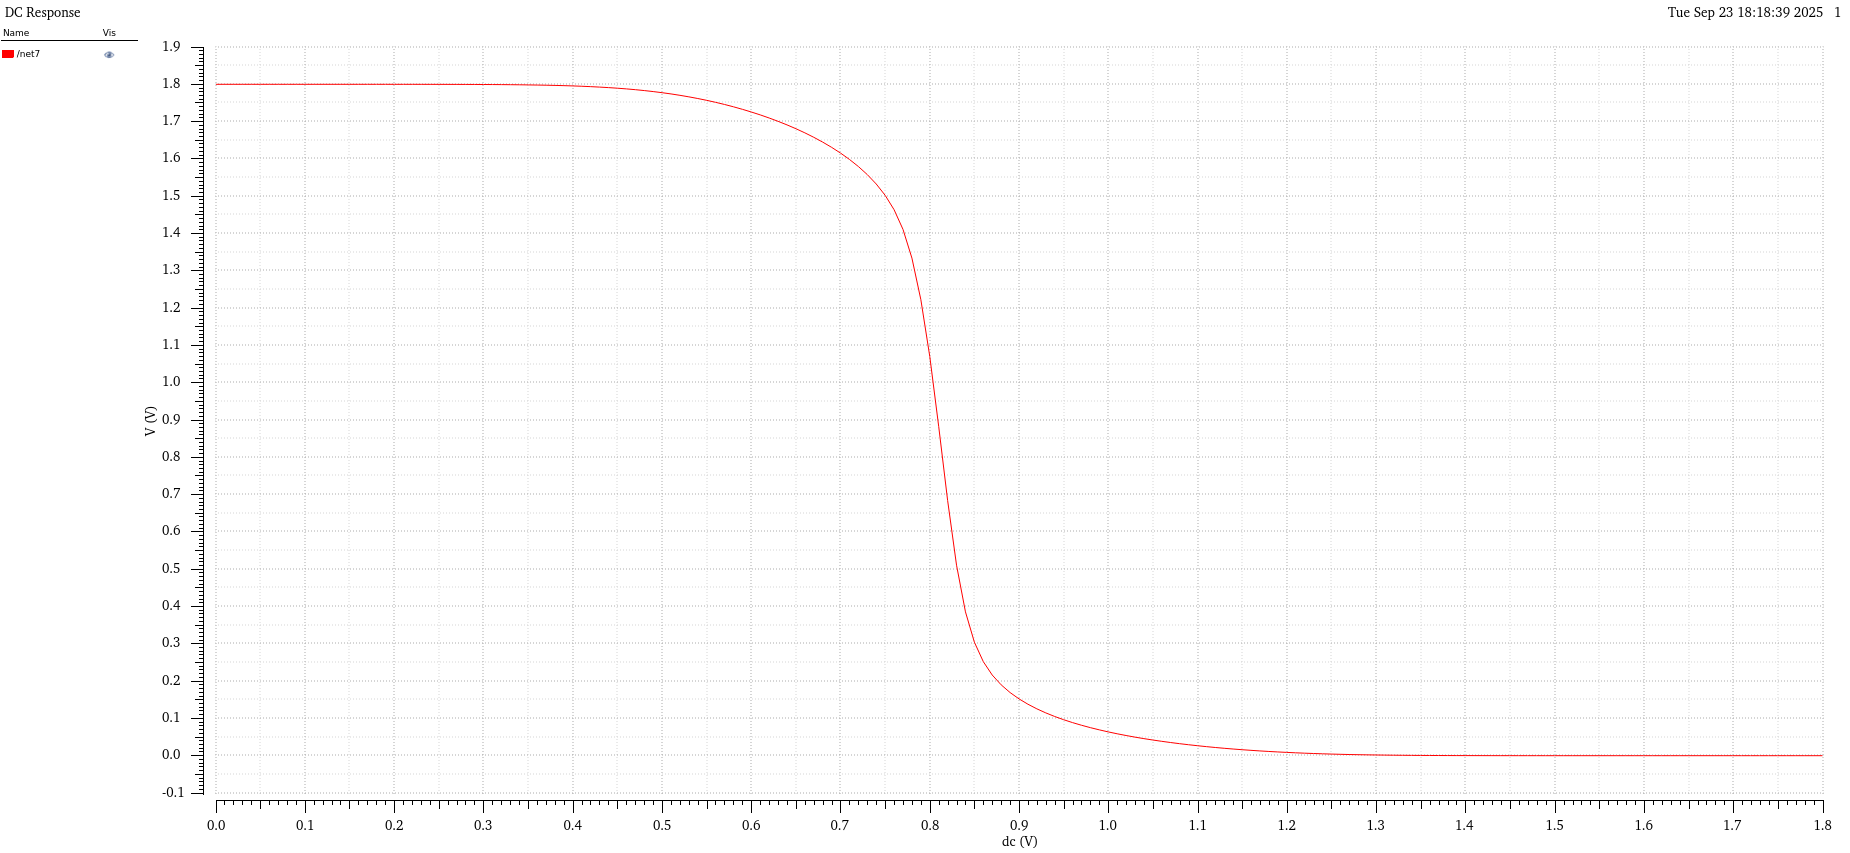
\includegraphics[width=\textwidth]{images/part1-vtc-curve.png}
		\caption{VTC Curve}
		\label{fig:vtc_curve}
	\end{subfigure}
	\hfill
	\begin{subfigure}{0.45\textwidth}
		\centering
		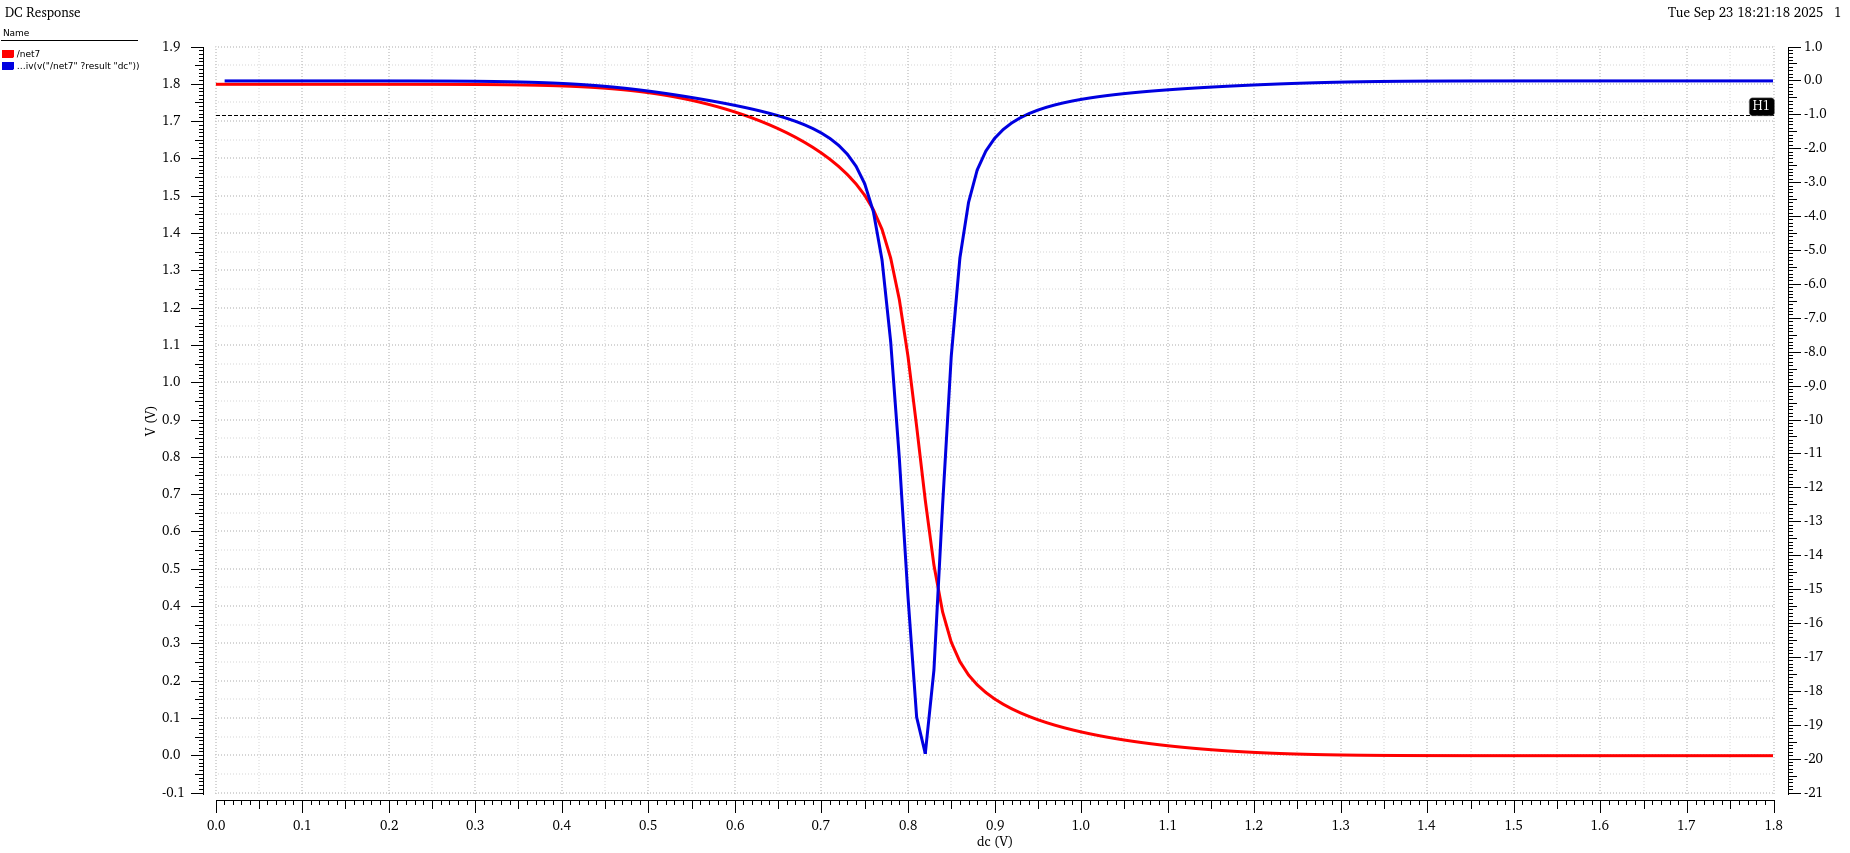
\includegraphics[width=\textwidth]{images/part1-vtc-curve-deriv.png}
		\caption{VTC Derivative}
		\label{fig:vtc_derivative}
	\end{subfigure}
	\caption{VTC Curves of the Basic CMOS Circuit}
\end{figure}

From the VTC curve, the following parameters were identified:
\begin{itemize}
	\item $V_{OH}$ = 1.8V = $V_{DD}$
	\item $V_{OL}$ = 0.2030279 mV $\neq$ GND
	\item $V_{IL}$ = 0.49974 V
	\item $V_{IH}$ = 1.19555 V
\end{itemize}

\section{Designing a Symmteric CMOS Inverter}
This next section of the lab required the design of the CMOS inverter to be symmetric. This was done by adjusting the width of the PMOS transistor from 660 nm to 1460nm. A straight line of $V_{out} = V_{in}$ was plotted on the VTC vurve to identify the width at which the PMOS VTC intersected this line. Upon the first iteration of the parametric analysis shown in Figure \ref{fig:parametric-analysis-1}, it was determined that the width of the PMOS should be between 1160nm and 1260nm. Figure \ref{fig:parametric-analysis-2} shows this portion of the graph zoomed in.
\begin{figure}[h!]
	\centering
	\begin{subfigure}{0.45\textwidth}
		\centering
		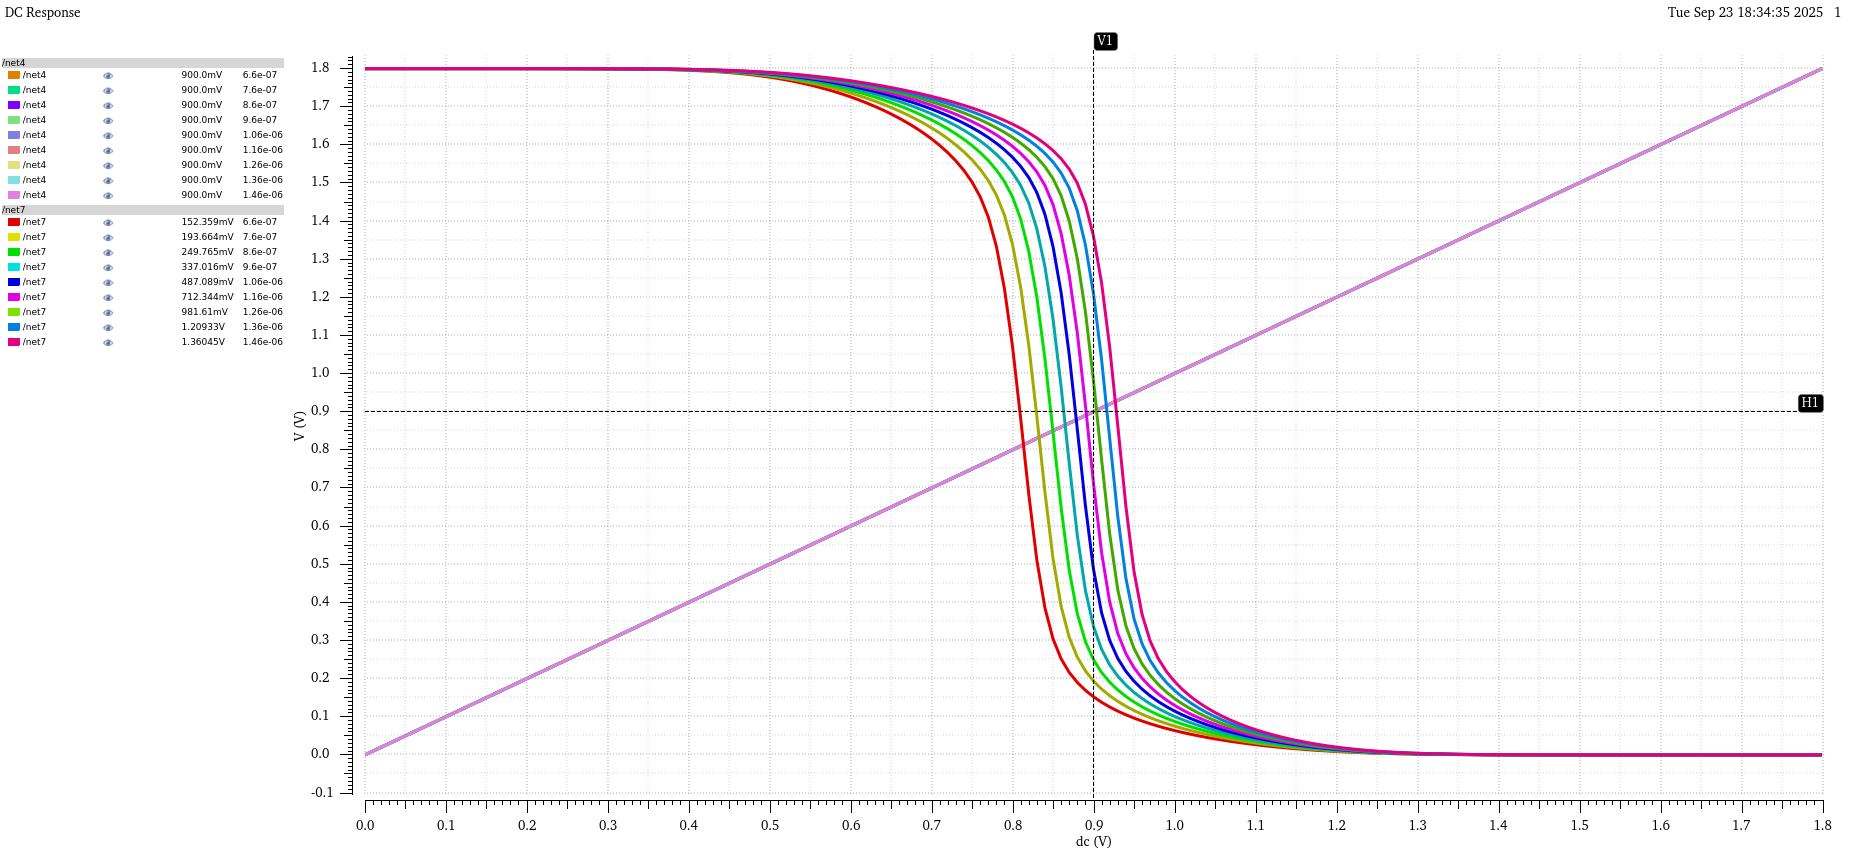
\includegraphics[width=\textwidth]{images/part2-width-variance-parametric-1.png}
		\caption{First round of parametric analysis}
		\label{fig:parametric-analysis-1}
	\end{subfigure}
	\hfill
	\begin{subfigure}{0.45\textwidth}
		\centering
		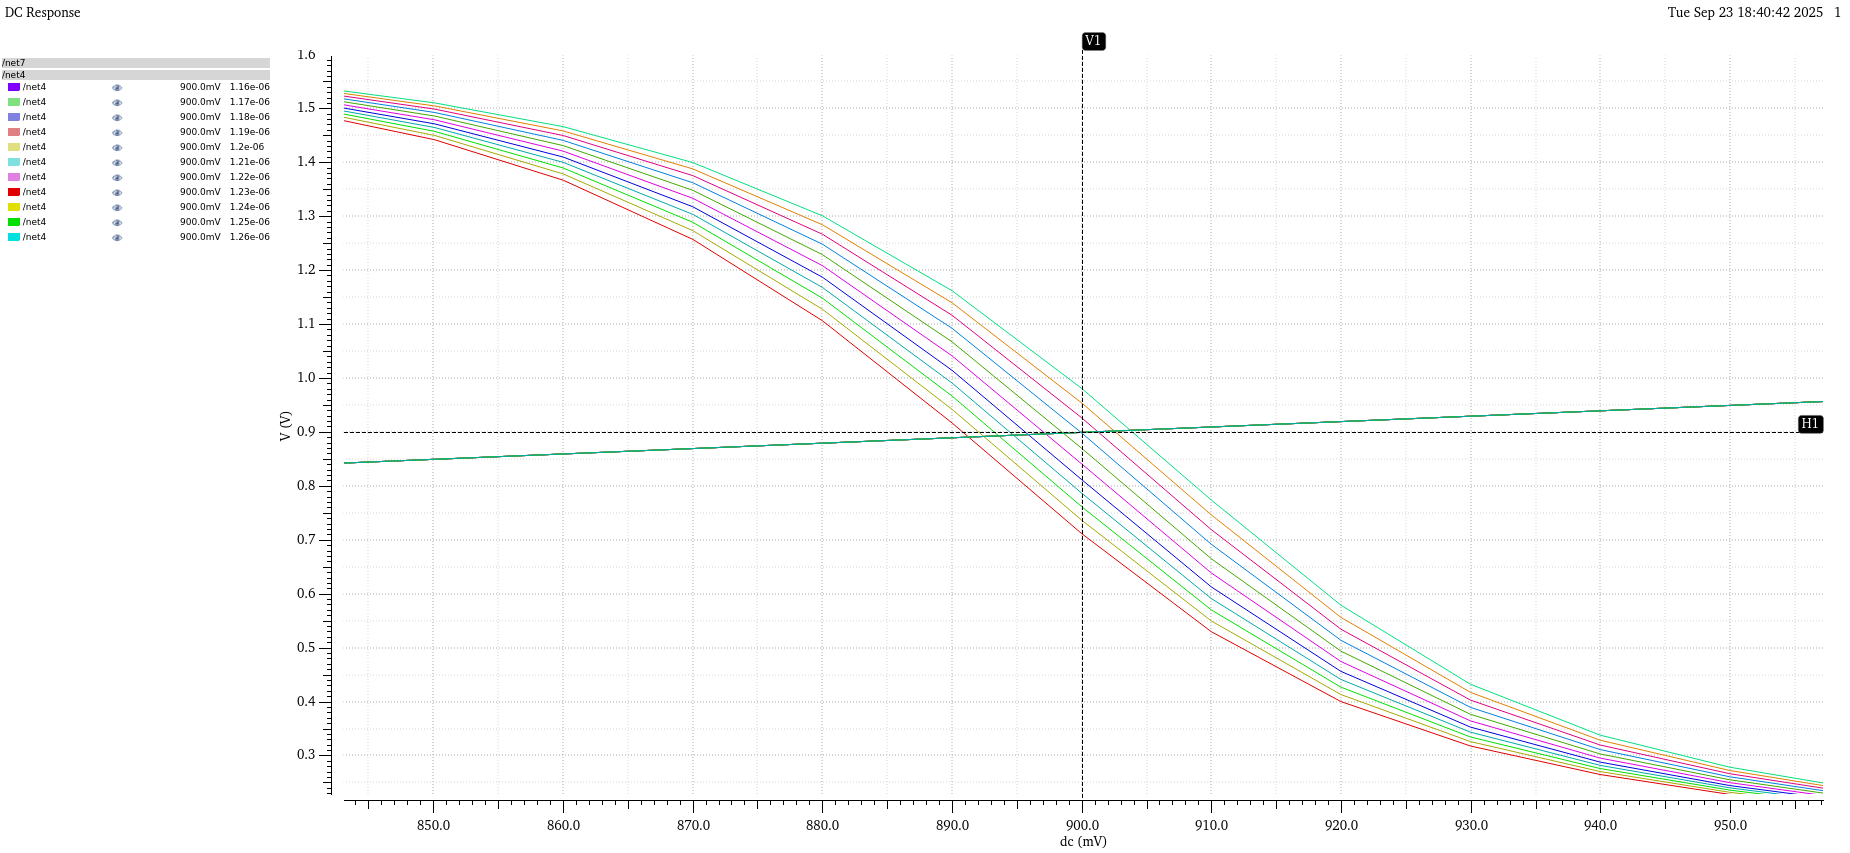
\includegraphics[width=\textwidth]{images/part2-width-variance-parametric-2.png}
		\caption{Zoomed in portion of the graph}
		\label{fig:parametric-analysis-2}
	\end{subfigure}
	\caption{Parametric analysis of PMOS width round 1}
\end{figure}

\newpage
Now, upon a second round of parametric analysis between the widths of 1160nm and 1260nm, the following graph in Figure \ref{fig:parametric-analysis-3} was obtained.
\begin{figure}[h!]
	\centering
	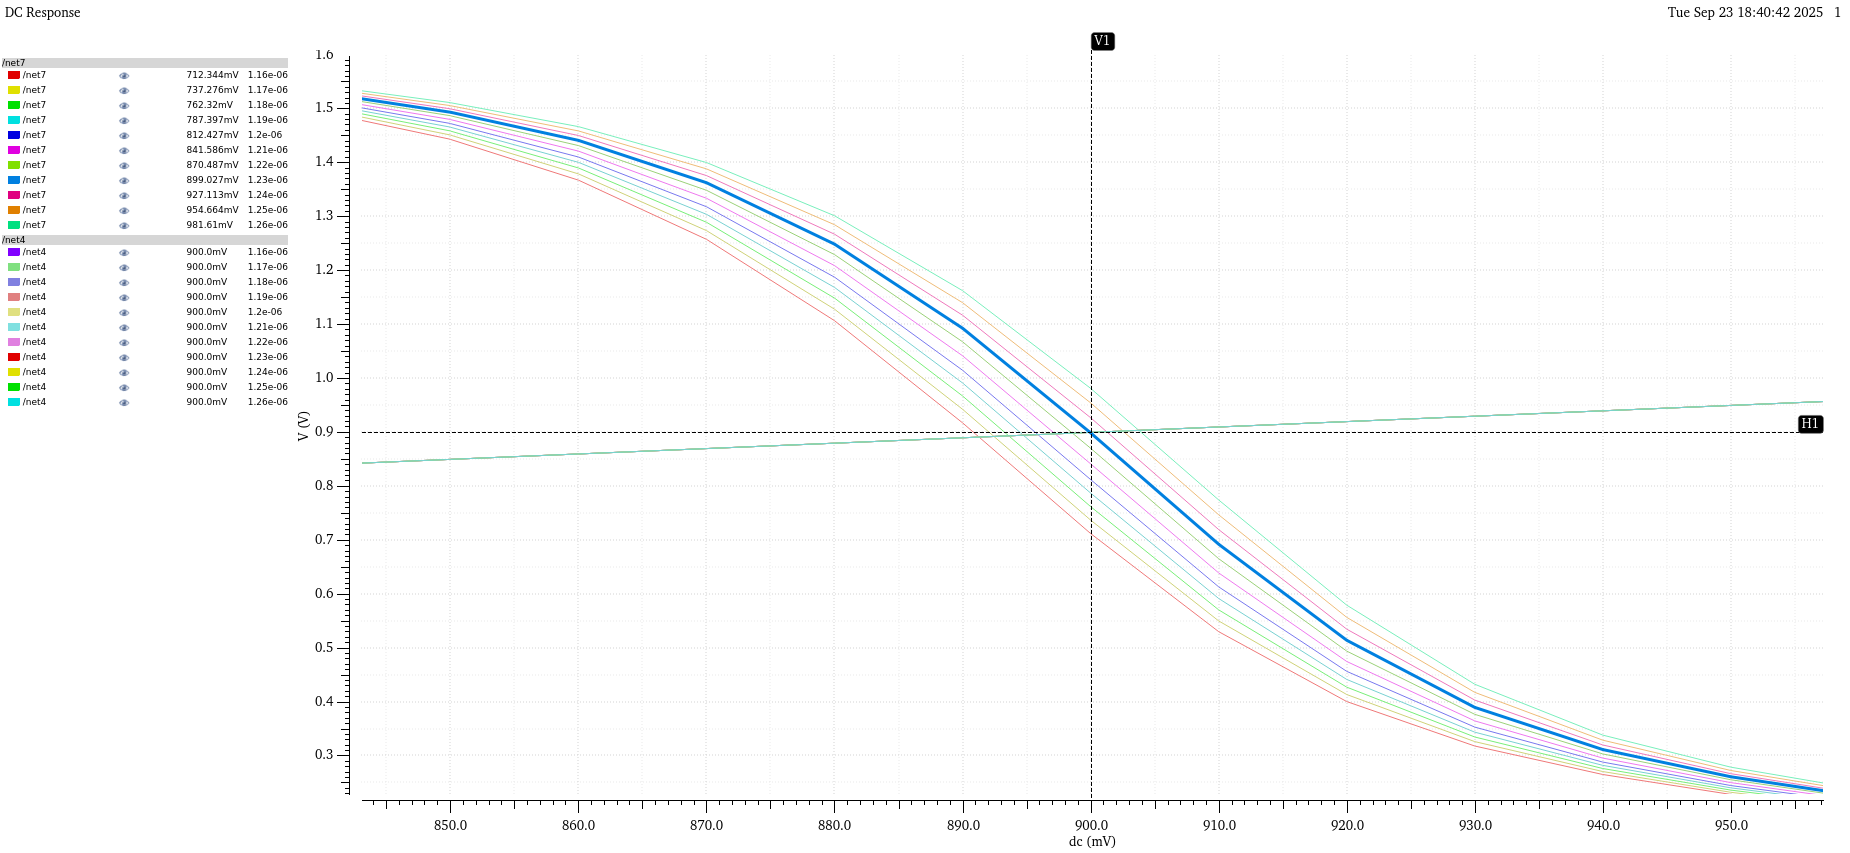
\includegraphics[width = 0.8\textwidth]{images/part2-width-variance-parametric-3.png}
	\caption{Second round of parametric analysis}
	\label{fig:parametric-analysis-3}
\end{figure}

This graph shows that the width of the PMOS should be 1230nm to obtain a symmetric CMOS inverter for this NMOS configuration. For the next part of this lab, that particular value was used.

\section{Transient Analysis of the Symmetric CMOS Inverter}
The final part of this lab involved performing a transient analysis of the symmetric CMOS inverter designed in the previous section. The input was a pulse wave with the following parameters:
\begin{itemize}
	\item V1 = 0V
	\item V2 = 1.8V
	\item Rise time = 0.1ns
	\item Fall time = 0.1ns
	\item Pulse width = 10ns
	\item Period = 20ns
\end{itemize}

A transient analysis without any output capacitance was performed first. The output of this analysis is shown in Figure \ref{fig:transient-no-cap}.
\begin{figure}[h!]
	\centering
	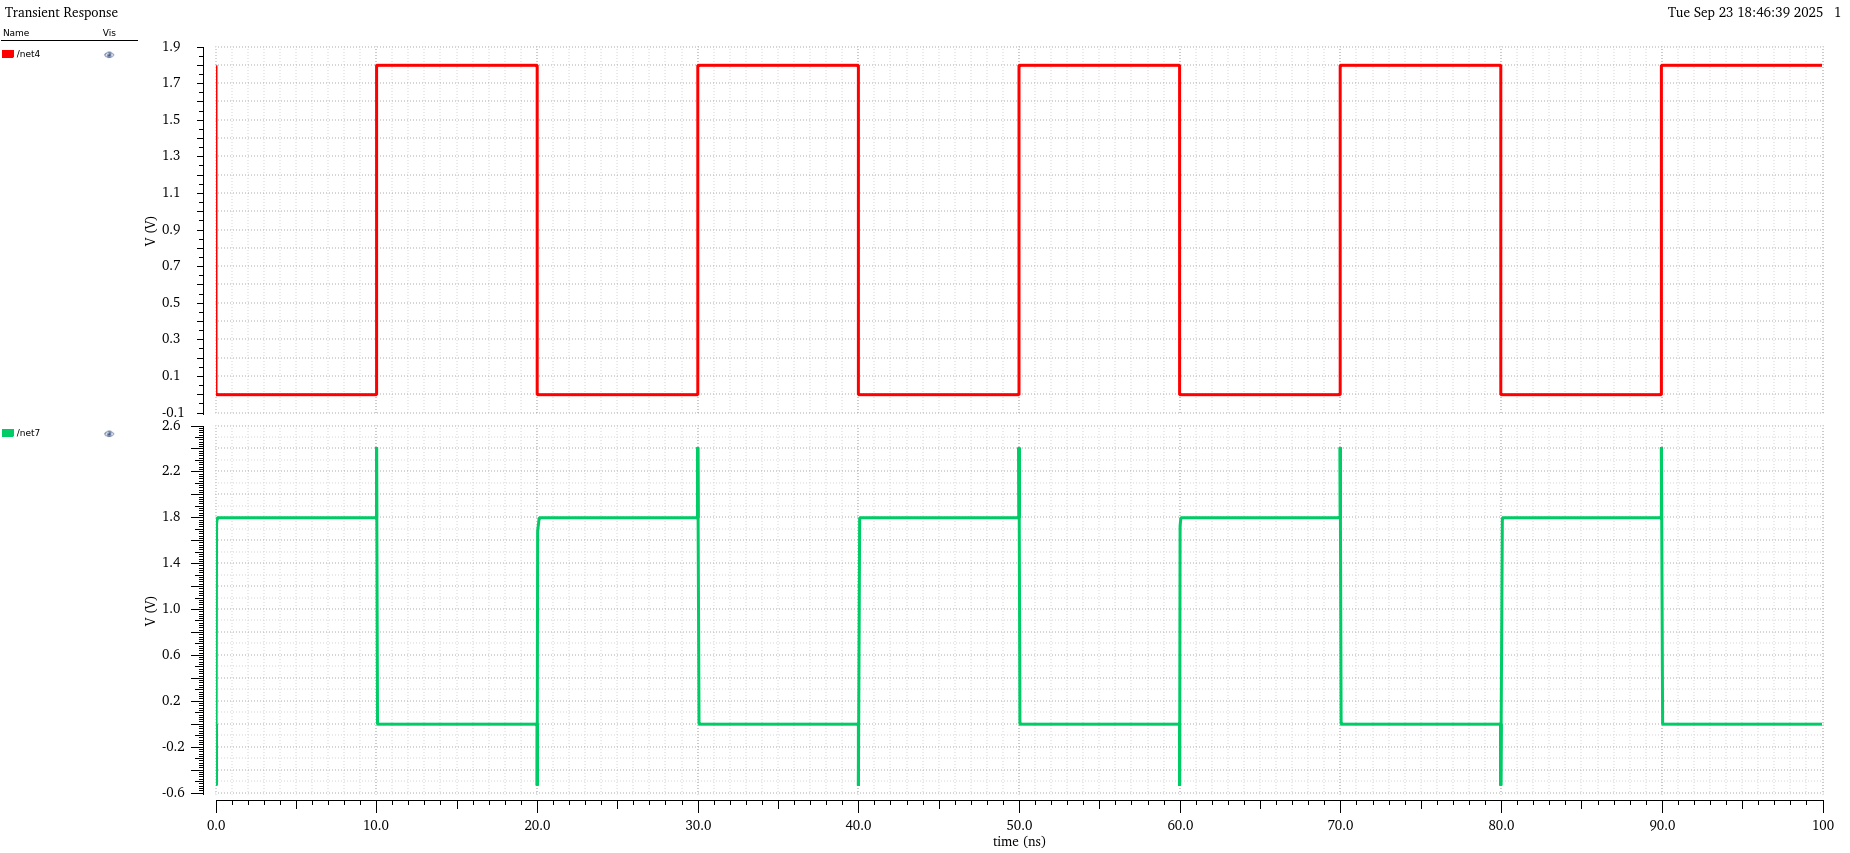
\includegraphics[width=\textwidth]{images/part3-no-cap.png}
	\caption{Transient Analysis without Output Capacitance}
	\label{fig:transient-no-cap}
\end{figure}

However, to account for the actual performacne of such a circuit, a $10fF$ capacitor was added to the output node. The output of this analysis is shown in Figure \ref{fig:transient-with-cap}.

\begin{figure}[h!]
	\centering
	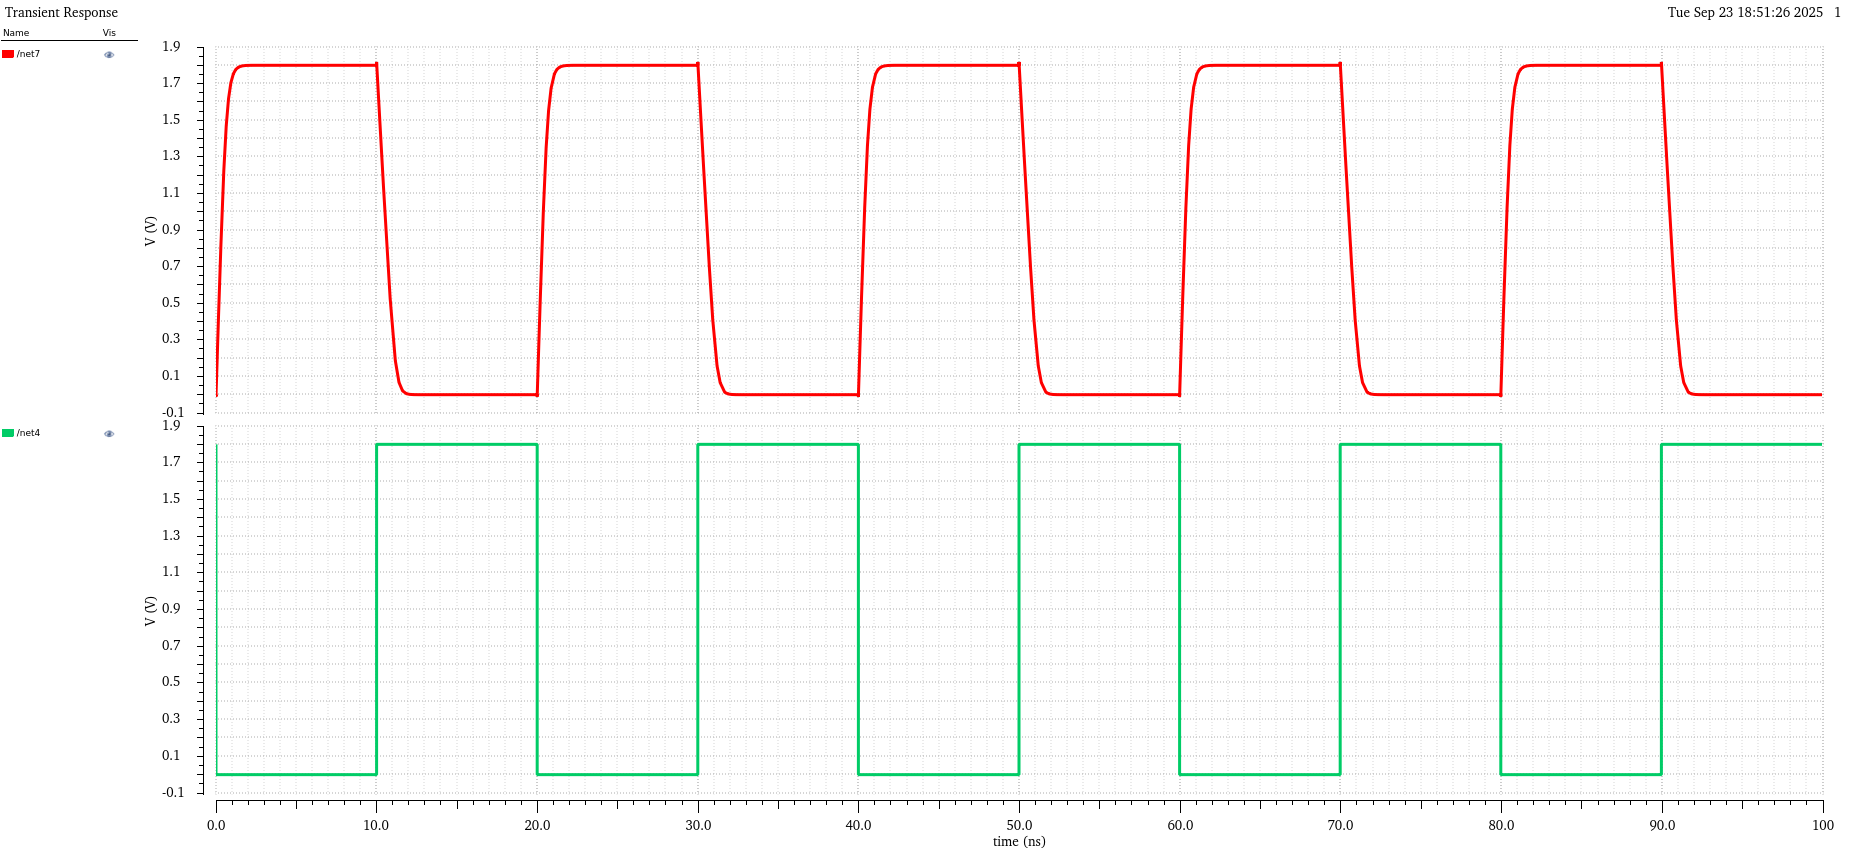
\includegraphics[width=\textwidth]{images/part3-with-cap.png}
	\caption{Transient Analysis with 10fF Output Capacitance}
	\label{fig:transient-with-cap}
\end{figure}
\end{document}

